[65 v\textsuperscript{o}] observationes requirant altitudines sideris\protect\index{Sachverzeichnis}{sidus} observandi aequales, aut observationem unicam, sed sideris\protect\index{Sachverzeichnis}{sidus} in summa altitudine positi, seu meridianum\protect\index{Sachverzeichnis}{meridianus} transeuntis. Unde nec Refractionum\protect\index{Sachverzeichnis}{refractio} error magnopere metuendus est hac methodo nostra. \edtext{Nam}{\lemma{nostra.}\Afootnote{ \textit{ (1) }\ Cum eni \textit{ (2) }\ Nam \textit{ L}}} \edtext{interdiu}{\lemma{}\Afootnote{interdiu \textit{ erg.} \textit{ L}}} solis\protect\index{Sachverzeichnis}{sol} supra horizontem altius evecti refractio\protect\index{Sachverzeichnis}{refractio} non est magni momenti. Et noctu si unum sidus apparet, apparent etiam plura, eaque diversae ascensionis, ac proinde refractionum\protect\index{Sachverzeichnis}{refractio} quoque differentium, ut proinde duo simul observari, et inde collatione facta error exterminari possit. \pend
\pstart Contra si solis\protect\index{Sachverzeichnis}{sol} ortus occasusque observandus est, vereor ne difficile sit verum ortus occasusque tempus reperire, quia constat solem\protect\index{Sachverzeichnis}{sol} \edtext{in horizonte sensibili libero mari definiti surgentem aut cadentem}{\lemma{solem}\Afootnote{ \textit{ (1) }\ in aperto mari surgentem aut cadentem \textit{ (2) }\ in [...] cadentem \textit{ L}}}, miram sui speciem iri, extremi marginis undis exhibere, ac falsa sui varieque detorta.\footnote{\textit{Gestrichene Marginalie:} Commodissimum autem est eligi stellam\protect\index{Sachverzeichnis}{stella} ejusdem paralleli\protect\index{Sachverzeichnis}{circulus parallelus} cum nostro, aut saltem vicini.} Imagine sibi ipsi jam \edtext{summerso}{\lemma{jam}\Afootnote{ \textit{ (1) }\ depresso \textit{ (2) }\ summerso \textit{ L}}}, \edtext{diu}{\lemma{}\Afootnote{diu \textit{ erg.} \textit{ L}}} superesse at postea etiam specie illa fallaci subito evanescente noctem celerrime ac velut de improviso ingruere, \edtext{brevissimo ac parum notabili Crepusculo}{\lemma{ingruere,}\Afootnote{ \textit{ (1) }\ Crepusculo exiguo admodum \textit{ (2) }\ brevissimo ac parum notabili Crepusculo \textit{ L}\ \hspace{10mm}20f.\hspace{5mm} \textit{ (1) }\ Uti \textit{ (2) }\ Commodissimum [...] vicini, \textbar\ eamque meridiano\protect\index{Sachverzeichnis}{meridianus} non nimis 5 vicinam. \textit{ gestr. } \textbar\ \textit{ L }}} interjecto, \edtext{praeterquam quod saepissime accidet ut una observatione facta, altera altitudinis aequalis ab aeris navisve\protect\index{Sachverzeichnis}{navis} statu impediatur.}{\lemma{}\Afootnote{praeterquam [...] impediatur. \textit{ erg.} \textit{ L }}} \pend \pstart \edtext{Turbare non debet quod hoc loco ad Inventionem Longitudinum\protect\index{Sachverzeichnis}{longitudo}, Latitudines\protect\index{Sachverzeichnis}{latitudo} inventas praerequirimus; nam et alioquin Latitudinum\protect\index{Sachverzeichnis}{latitudo} quoque inventio jam tum necessaria est ad cursum navis\protect\index{Sachverzeichnis}{navis} gubernandum, et ut Latitudo\protect\index{Sachverzeichnis}{latitudo} sine Longitudine\protect\index{Sachverzeichnis}{longitudo}, ita contra Longitudo\protect\index{Sachverzeichnis}{longitudo} quoque sine latitudine\protect\index{Sachverzeichnis}{latitudo} non sufficit. Ut taceam hoc loco spem esse magnam, inveniri posse, aut ad perfectionem deduci quam primum inventionem Latitudinis\protect\index{Sachverzeichnis}{latitudo} seu elevationis Poli\protect\index{Sachverzeichnis}{elevatio!poli} universalem, ab omni observatione coelesti, ac proinde aeris marisque injuria independentem, de quo alias fusius dicendi locus erit.}{\lemma{}\Afootnote{Turbare [...] ; nam  \textbar\ et \textit{ erg.}\ \textbar\ alioquin [...] posse, \textit{ (1) }\ et \textit{ (2) }\ aut ad [...] Poli \textbar\ universalem \textit{ erg.}\ \textbar\ , ab [...] erit. \textit{ erg.} \textit{ L}}} Problema ergo meum ita concipitur: \edtext{\textso{Data Latitudine $\langle$l$\rangle$oci navis Horologioque exacto, et accedente}}{\lemma{\textso{Data}}\Afootnote{ \textit{ (1) }\ \textso{Horologio}\protect\index{Sachverzeichnis}{horologium|textit}\textso{ exacto, dataque} \textit{ (2) }\ \textso{Latitudine }[...]\textso{ accedente} \textit{ L}}}\textso{ unica, quacunque, }\textso{sideris}\protect\index{Sachverzeichnis}{sidus} \textso{ (motus explorati,) }\edtext{\textso{cujuscunque (in horizonte navis motum satis sensibilem habentis, seu polo non nimis vicini)}}{\lemma{\textso{cujuscunque}}\Afootnote{\textit{ (1) }\ \textso{(inprimis }\textso{meridiano}\protect\index{Sachverzeichnis}{meridianus|textit} \textit{ (2) }\ \textso{meridiano}\protect\index{Sachverzeichnis}{meridianus|textit}\textso{ non nimis vicini} \textit{ (3) }\ \textso{(in }[...]\textso{ vicini)} \textit{ erg.} \textit{ L}}}\textso{ observatione Longitudines}\protect\index{Sachverzeichnis}{longitudo}\textso{, ac }\edtext{\textso{per consequens}}{\lemma{\textso{ac}}\Afootnote{ \textit{ (1) }\ \textso{quod idem est} \textit{ (2) }\ \textso{per consequens} \textit{ L}}}\textso{ locum }\textso{navis}\protect\index{Sachverzeichnis}{navis}\textso{, reperire.}\pend \clearpage
\pstart \edtext{Problema jam propositum ita solvetur.}{\linenum{74|15||75|1||}\lemma{\textso{reperire.}}\Afootnote{ \textit{ (1) }\ Hoc ita fiet: Dato Horologio\protect\index{Sachverzeichnis}{horologium|textit} exacto datur locus sideris \protect\index{Sachverzeichnis}{sidus|textit} in coelo, quodcunque  sit, in \textit{(a)}\ ordin \textit{(b)}\ respectu, ad locum \textit{(aa)}\ , ubi ho \textit{(bb)}\ discessus,  ad quem horologium\protect\index{Sachverzeichnis}{horologium|textit} direximus, qui \textit{ (2) }\ Cum \textit{ (3) }\ Datur enim  hora loci discessus, ac per consequens situs omnium siderum\protect\index{Sachverzeichnis}{sidus|textit}, \textit{(a)}\ qui \textit{(b)}\ posito quod nobis loci discessus latitudo\protect\index{Sachverzeichnis}{latitudo|textit} et longitudo\protect\index{Sachverzeichnis}{longitudo|textit} cognita sit. Datur vero praeterea circulus aequatori\protect\index{Sachverzeichnis}{aequator} parallelus\protect\index{Sachverzeichnis}{circulus parallelus|textit} in quo navis\protect\index{Sachverzeichnis}{navis|textit} nunc versatur, Latitudine\protect\index{Sachverzeichnis}{latitudo|textit} quippe navis\protect\index{Sachverzeichnis}{navis|textit} data. Ac datur denique angulus quem facit sidus\protect\index{Sachverzeichnis}{sidus|textit} cujus aspectus nobis conceditur (et cujus per priora, locum praesentem in mundo, scimus) ad horizontem navis\protect\index{Sachverzeichnis}{navis|textit}, \textit{(aa)}\ seu ad circulum parallelum navis\protect\index{Sachverzeichnis}{navis|textit}. Idem enim est angulus ad horizontem navis\protect\index{Sachverzeichnis}{navis|textit}, et ad \textit{(aaa)}\ parallelum \textit{(bbb)}\ tangentem circuli paralleli navis\protect\index{Sachverzeichnis}{navis|textit}. Quia \textit{(bb)}\ seu ad tangentem globi telluris\protect\index{Sachverzeichnis}{tellus|textit} in puncto navis\protect\index{Sachverzeichnis}{navis|textit}, aut ad radium ductum ex centro terrae\protect\index{Sachverzeichnis}{terra|textit} in punctum navis\protect\index{Sachverzeichnis}{navis|textit}. \textit{(aaa)}\ Facit aut \textit{(bbb)}\ Cognitum autem est quem angulum faciat Circulus Parallelus datus ejusve tangens, aut radius ad radium aut tangentem telluris\protect\index{Sachverzeichnis}{tellus|textit} a quo producto tangitur aut secatur. Ergo \textbar\ cognoscetur, \textit{ erg.}\ \textbar\ quem angulum faciat linea ex sidere\protect\index{Sachverzeichnis}{sidus|textit} ducta seu radius sideris \protect\index{Sachverzeichnis}{sidus|textit} ad Parallelum\protect\index{Sachverzeichnis}{circulus parallelus|textit}. Jam \textit{(aaaa)}\ idem punctum cognitum \textit{(bbbb)}\ ex uno puncto extra circulum (aut saltem extra circuli centrum) posito ad eundem circulum non possunt duci duae lineae eundem angulum facientes. \textit{(aaaaa)}\ Est ergo \textit{(bbbbb)}\ Determinato ergo circulo, et puncto extra circulum, $\langle$--$\rangle$ $\langle$et$\rangle$ angulo \textit{(aaaaa-a)}\ puncti \textit{(bbbbb-b)}\ lineae circulum puncto connectentis ad circulum (id est ad circuli radium vel tangentem) determinatum erit punctum in circulo, ad quod linea connectens facit angulum datum. \textit{ (4) }\ Hoc ita fiet \textit{ (5) }\ Problema jam propositum ita solvetur \textit{ L}}}\pend
   \clearpage
   \pstart \noindent \textit{[Folgende Zeichnungen sind \"uber die rechte Spalte verteilt und k\"onnen nicht eindeutig zugeordnet werden:]}\\
   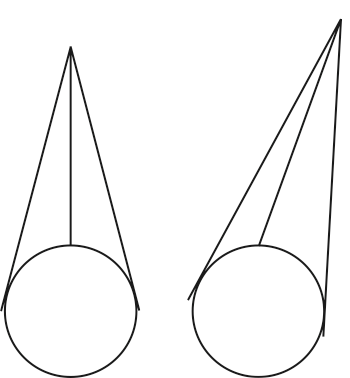
\includegraphics[width=0.25\textwidth]{images/35_15_6_65vfig1u2}
   \hspace{10mm}
   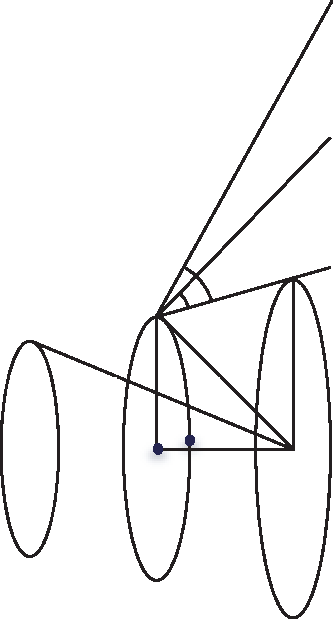
\includegraphics[width=0.35\textwidth]{images/35_15_6_65vfig3}
   \hspace{10mm}
   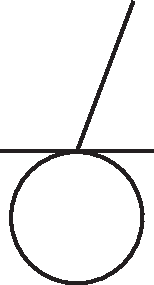
\includegraphics[width=0.1\textwidth]{images/35_15_6_65vfig4}
   \\
   \hspace{7mm} \textit{[Fig. 2]}\hspace{6mm}\textit{[Fig. 3]} \hspace{20mm}\textit{[Fig. 4, gestrichen]}\hspace{20mm}\textit{[Fig. 5]}\pend
   \vspace{5mm}
   \pstart \noindent \textit{[Nebenrechnungen, die ebenfalls nicht eindeutig zugeordnet werden k\"onnen:]}\\ \vspace{1.0ex} \begin{center}
$\begin{array}{l} \hspace{5.5pt}600\\\hspace{5.5pt}6\\\overline{3600}\end{array}$ \hspace{10mm}
$\begin{array}{l} \hspace{11pt}36000\\\hspace{11pt}36\\\hspace{5.5pt}\underline{\overline{216000}}\\108\\\overline{1296000}\end{array}$
\hspace{10mm}
$\begin{array}{l} \hspace{5.5pt}3600\\\hspace{11pt}6\\\overline{21600}\end{array}$
\end{center}\pend
